\chapter{Ein Kapitel}

\section{Ein Abschnitt}

\subsection{Ein Unterabschnitt}

\section{Pix2Pix}
Pix2Pix, initiiert von Isola et al., hat sich als zentrales Framework für Bild-zu-Bild-Übersetzungen auf der Basis von bedingten generativen adversariellen Netzwerken (cGANs) etabliert. Es ermöglicht die Erstellung einer abstrakten Abbildung von einem Eingangsbild zu einem korrespondierenden Ausgangsbild und bewältigt dabei eine vielfältige Palette an Bildübersetzungsaufgaben, wie die Transformation von Skizzen in realistische Bilder oder die Konvertierung von Tages- zu Nachtaufnahmen. \newline
Pix2Pix fungiert hier als Generative Adversarial Network (GAN), spezialisiert auf diverse Formen der Bildübersetzung. Darunter fallen die Umwandlung von Schwarz-Weiß-Fotos in Farbbilder, die Transformation von Skizzen in realistische Bilder, und relevant für diese Arbeit, die Konvertierung von Satellitenbildern in kartographische Darstellungen, ähnlich den Visualisierungen von Google Maps. \newline	Die Architektur von Pix2Pix besteht aus einem Generator und einem Diskriminator. Der Generator, der eine U-Net-Architektur verwendet, besteht aus einem Encoder und einem Decoder. Der Encoder komprimiert das Eingangsbild schrittweise zu einer niedrigdimensionalen Repräsentation, während der Decoder diese dazu nutzt, das Ausgangsbild zu rekonstruieren. Skip-Verbindungen zwischen Encoder und Decoder helfen dabei, sowohl globale als auch lokale Informationen im generierten Bild zu bewahren. \newline
Der Diskriminator nimmt die Form eines PatchGAN-Modells an und bewertet Patches des Bildes, indem er die Wahrscheinlichkeit für die Echtheit jedes Patches ausgibt. Dies ermöglicht die Anwendung des Diskriminators auf Bilder unterschiedlicher Größen. Im Zuge des adversariellen Trainingsprozesses passen sowohl der Generator als auch der Diskriminator ihre Fähigkeiten fortlaufend an. Während der Generator lernt, immer realistischere Übersetzungen zu erzeugen, wird der Diskriminator stetig besser darin, zwischen echten und generierten Bildern zu unterscheiden.
 

\subsection{Pix2Pix-Kernkonzepte}
Die Bildverarbeitung hat in den letzten Jahren durch den Einsatz tiefer neuronaler Netzwerke erhebliche Fortschritte gemacht. Im Mittelpunkt vieler dieser Fortschritte steht die U-Net-Architektur, die speziell für die Bildsegmentierung entwickelt wurde. Diese Architektur zeichnet sich durch ihre angeklügelte Kombination aus Encoder- und Decoder- Strukturen sowie durch den Einsatz von Skip-Verbindungen aus.
 \newline
Bei der Encoder-Decoder-Struktur handelt es sich um einen Ansatz, bei dem das Eingangsbild zunächst durch den Encoder schrittweise reduziert wird. Dieser Prozess dient dazu, wesentliche Merkmale des Bildes zu erfassen. Anschließend wird das Bild durch den Decoder wiederhergestellt, indem die zuvor extrahierten Merkmale verwendet werden. Während dieser Prozesse besteht jedoch das Risiko des Informationsverlustes, insbesondere in den tieferen Schichten des Netzwerks.
Um dieses Problem zu adressieren, führt die U-Net-Architektur Skip-Verbindungen ein. Diese direkten Verbindungen zwischen korrespondierenden Schichten des Encoders und Decoders sorgen dafür, dass Detailinformationen nicht verloren gehen. Genauer gesagt, ermöglichen diese Verbindungen den direkten Informationsfluss zwischen jeweils äquivalenten Schichten, wodurch die Rekonstruktion des Bildes im Decoder mit einer höheren Genauigkeit erfolgt. \newline
Die Bedeutung von Skip-Verbindungen zeigt sich insbesondere in Anwendungen wie der Bild-zu-Bild-Übersetzung. Hier muss oft ein Bild mit niedriger Auflösung in ein Bild mit hoher Auflösung überführt werden, ohne dass Details verloren gehen. Die U-Net-Architektur, die angereichert mit diesen Verbindungen ist, ermöglicht daher eine feinere Rekonstruktion, die sowohl globale als auch lokale Informationen berücksichtigt. \newline
Somit kann die U-Net-Architektur durch ihre Kombination aus Encoder-Decoder-Struktur und Skip-Verbindungen ein effektives Werkzeug für die Bildsegemtierung darstellen. Ihre Fähigkeit, sowohl globale Muster als auch feine Details zu berücksichtigen, macht sie zu einer bevorzugten Wahl für viele Bildverarbeitungsaufgaben. \newline
In Abbildung \ref{fig:unet} ist die typische U-Net-Architektur dargestellt. Die linke Seite des ''U'' repräsentiert den Encoder-Teil, der das Eingangsbild schrittweise reduziert und wesentliche Merkmale extrahiert. Die rechte Seite repräsentiert den Decoder-Teil, der das Bild mithilfe der extrahierten Merkmale rekonstruiert. Die horizontalen Linien repräsentieren die Skip-Verbindungen, die sicherstellen, dass Detailinformationen zwischen den korrespondierenden Schichten des Encoder und Decoders direkt übertragen werden. \newline 
In der Pix2Pix Technologie dient diese U-Net-Architektur als Generator. Er ist das zentrale Element, das für die Bild-zu-Bild-Übersetzung verantwortlich ist. Die Wahl der U-Net-Struktur für den Generator liegt in ihrer Fähigkeit, feinere Details und Kontextinformationen aus dem Eingangsbild beizubehalten, was für die Bild-zu-Bild-Übersetzung von entscheidender Bedeutung ist. Die Encoder-Decoder-Struktur des U-Net ermöglicht es dem Generator, den globalen Kontext des Bildes zu erfassen, während die Skip-Verbindungen sicherstelle, dass auch lokale Details im resultierenden Bild berücksichtigt werden.

\begin{figure}[h]
	\centering
	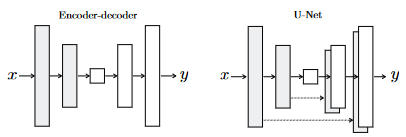
\includegraphics[width=0.7\linewidth]{./images/unet.png}
	\caption{Schematische Darstellung der U-Net-Architektur. Die Architektur besteht aus einem Encoder-Teil (links), einem Decoder-Teil (rechts) und Skip-Verbindungen zwischen korrespondierenden Schichten.}
	\label{fig:unet}
\end{figure}


